\section{eo\-IBEASorting$<$ EOT, Fitness $>$ Class Template Reference}
\label{classeoIBEASorting}\index{eoIBEASorting@{eoIBEASorting}}
Functor The sorting phase of IBEA (Indicator-Based Evolutionary Algorithm) without uncertainty Adapted from the Zitzler and K\~{A}�nzli paper \char`\"{}Indicator-Based Selection in Multiobjective Search\char`\"{} (2004) Of course, Fitness needs to be an {\bf eo\-Pareto\-Fitness} object.  


{\tt \#include $<$eo\-IBEA.h$>$}

Inheritance diagram for eo\-IBEASorting$<$ EOT, Fitness $>$::\begin{figure}[H]
\begin{center}
\leavevmode
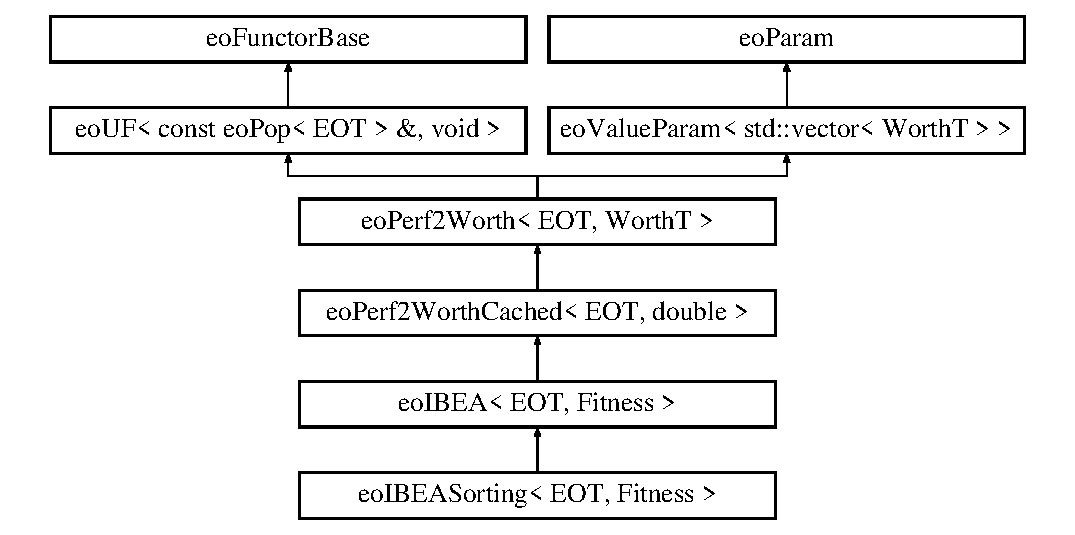
\includegraphics[height=6cm]{classeoIBEASorting}
\end{center}
\end{figure}
\subsection*{Public Member Functions}
\begin{CompactItemize}
\item 
{\bf eo\-IBEASorting} ({\bf eo\-Binary\-Quality\-Indicator}$<$ Fitness $>$ $\ast$\_\-I, const double \_\-kappa)
\begin{CompactList}\small\item\em constructor \item\end{CompactList}\end{CompactItemize}
\subsection*{Private Member Functions}
\begin{CompactItemize}
\item 
void {\bf set\-Bounds} (const {\bf eo\-Pop}$<$ EOT $>$ \&\_\-pop)
\begin{CompactList}\small\item\em computation and setting of the bounds for each objective \item\end{CompactList}\item 
void {\bf fitnesses} (const {\bf eo\-Pop}$<$ EOT $>$ \&\_\-pop)
\begin{CompactList}\small\item\em computation and setting of the fitness for each individual of the population \item\end{CompactList}\end{CompactItemize}
\subsection*{Private Attributes}
\begin{CompactItemize}
\item 
double {\bf kappa}\label{classeoIBEASorting_de45fa88a6b6fc70896a0dbfffdb3dc7}

\begin{CompactList}\small\item\em scaling factor kappa \item\end{CompactList}\end{CompactItemize}


\subsection{Detailed Description}
\subsubsection*{template$<$class EOT, class Fitness = typename EOT::Fitness$>$ class eo\-IBEASorting$<$ EOT, Fitness $>$}

Functor The sorting phase of IBEA (Indicator-Based Evolutionary Algorithm) without uncertainty Adapted from the Zitzler and K\~{A}�nzli paper \char`\"{}Indicator-Based Selection in Multiobjective Search\char`\"{} (2004) Of course, Fitness needs to be an {\bf eo\-Pareto\-Fitness} object. 



Definition at line 94 of file eo\-IBEA.h.

\subsection{Constructor \& Destructor Documentation}
\index{eoIBEASorting@{eo\-IBEASorting}!eoIBEASorting@{eoIBEASorting}}
\index{eoIBEASorting@{eoIBEASorting}!eoIBEASorting@{eo\-IBEASorting}}
\subsubsection{\setlength{\rightskip}{0pt plus 5cm}template$<$class EOT, class Fitness = typename EOT::Fitness$>$ {\bf eo\-IBEASorting}$<$ EOT, Fitness $>$::{\bf eo\-IBEASorting} ({\bf eo\-Binary\-Quality\-Indicator}$<$ Fitness $>$ $\ast$ {\em \_\-I}, const double {\em \_\-kappa})\hspace{0.3cm}{\tt  [inline]}}\label{classeoIBEASorting_7a35d760e84a98fd7a47966c50e3af66}


constructor 

\begin{Desc}
\item[Parameters:]
\begin{description}
\item[{\em eo\-Binary\-Quality\-Indicator$<$EOT$>$$\ast$}]\_\-I the binary quality indicator to use in the selection process \item[{\em double}]\_\-kappa scaling factor kappa \end{description}
\end{Desc}


Definition at line 106 of file eo\-IBEA.h.

References eo\-IBEASorting$<$ EOT, Fitness $>$::kappa.

\subsection{Member Function Documentation}
\index{eoIBEASorting@{eo\-IBEASorting}!setBounds@{setBounds}}
\index{setBounds@{setBounds}!eoIBEASorting@{eo\-IBEASorting}}
\subsubsection{\setlength{\rightskip}{0pt plus 5cm}template$<$class EOT, class Fitness = typename EOT::Fitness$>$ void {\bf eo\-IBEASorting}$<$ EOT, Fitness $>$::set\-Bounds (const {\bf eo\-Pop}$<$ EOT $>$ \& {\em \_\-pop})\hspace{0.3cm}{\tt  [inline, private, virtual]}}\label{classeoIBEASorting_02c7346d6aa62f3e3af20cc6ac3ee1d9}


computation and setting of the bounds for each objective 

\begin{Desc}
\item[Parameters:]
\begin{description}
\item[{\em const}]eo\-Pop$<$EOT$>$\& \_\-pop the population \end{description}
\end{Desc}


Implements {\bf eo\-IBEA$<$ EOT, Fitness $>$} {\rm (p.\,\pageref{classeoIBEA})}.

Definition at line 134 of file eo\-IBEA.h.\index{eoIBEASorting@{eo\-IBEASorting}!fitnesses@{fitnesses}}
\index{fitnesses@{fitnesses}!eoIBEASorting@{eo\-IBEASorting}}
\subsubsection{\setlength{\rightskip}{0pt plus 5cm}template$<$class EOT, class Fitness = typename EOT::Fitness$>$ void {\bf eo\-IBEASorting}$<$ EOT, Fitness $>$::fitnesses (const {\bf eo\-Pop}$<$ EOT $>$ \& {\em \_\-pop})\hspace{0.3cm}{\tt  [inline, private, virtual]}}\label{classeoIBEASorting_af613f862a58b402d88958b0e290e810}


computation and setting of the fitness for each individual of the population 

\begin{Desc}
\item[Parameters:]
\begin{description}
\item[{\em const}]eo\-Pop$<$EOT$>$\& \_\-pop the population \end{description}
\end{Desc}


Implements {\bf eo\-IBEA$<$ EOT, Fitness $>$} {\rm (p.\,\pageref{classeoIBEA})}.

Definition at line 162 of file eo\-IBEA.h.

The documentation for this class was generated from the following file:\begin{CompactItemize}
\item 
eo\-IBEA.h\end{CompactItemize}
